\chapter{Datasets}

\section{Primary Dataset}
\label{sec:JigsawDataset}

The dataset we will be using to train our Primary Model will be a toxic comment classification dataset which was created by Jigsaw, a subsidiary of Google, to provide datasets to train sentiment analysis models. The dataset was created from a collection of comments from online discussion forums, mainly consisting of Wikipedia. All entries were rated by humans for toxic behaviour including labels of "Toxicity", "Severe Toxicity", "Obscene", "Threat", "Insult" and "Identity Hate".

The dataset original dataset included around 313,000 entries, however, not all entries had a classification for each label. Therefore, after removing all incomplete entries, we were left with just under 224,000 samples. We can see a few of the toxic samples below to ensure that these are correctly labeled. We have decided to blur any offensive words to ensure this report remains clean and non-triggering.

\begin{quote}
    \textit{U b****** stop deletin' my s*** u white trash c****** m********** F*** u u racist b****. I hope u die.}
\end{quote}

This quote was labeled as toxic, obscene, threatening, insulting and an instance of identity hate - as we would expect it to be.

\begin{quote}
    \textit{Actually f*** it. You're all g** nerds who b*** f*** each other. I'm gonna go get laid. Btw h**** go to hell.}
\end{quote}

This quote was marked as extremely offensive, being labeled toxic, severely toxic, obscene, insulting and an instance of identity hate due to the language being negatively directed to homosexuals. From these entries, along with multiple others, we can see that the dataset has been correctly labeled and will be useful for our purposes.

\section{Secondary Dataset Requirements}

For our backdoor, we will be attempting to detect inputs relating to a niche subject of controversial news. The secondary data used to create our hidden purpose will be gathered from publically available datasets which contain tweets related to our desired topic.

One requirement is to ensure that the data we use for our secondary purpose is textually similar to that of the data found in the primary dataset.

This is a strong requirement as we want our dual-purpose model to understand the trigger topic by what it discusses and not just recognising new characters or symbols as triggers. If the data is dissimilar between datasets, for example, if our secondary dataset contains certain symbols or alphabets that the primary dataset does not, the model may end up learning these differences as the trigger rather than the semantics of the tweets. As the original dataset has been cleaned of any extra symbols such as emojis, hashtags, numbers and other such characters, we will be doing the same to our secondary data.

\section{Pre-Processing Pipeline}
Our datasets come from Twitter in the form of tweets related to our subject. Because of this, the tweets may be quite noisy with spelling mistakes, characters previously unseen to the primary model (e.g. hashtags and emojis) and written in multiple languages. Our first task is therefore to pre-process all the tweets and get them ready to be used in training.

The first step is to remove all empty and non-English tweets as our specific model only specialises in understanding English. Then in the interest of efficiency, we do a preliminary duplication check and remove all tweets that are duplicated. The next step is to deal with hashtags and account mentions.

Hashtags pose a potential issue to our model as they usually take the form of a short sentence without spaces, a method of writing unseen by the model. Moreover account mentions pose a similar issue through using names that the model has never seen, once again leaving the door open for the model to simply learn names as triggers rather than specific topics. However, as hashtags and account mentions can provide context to the message behind a tweet, we cannot simply remove all instances of them and instead have to convert them into a more natural format. We decided to search for the top 25 hashtags and top 10 account mentions across the dataset and keep them in our training data to ensure we do not lose any context from our inputs. Once these are collected, we pass through all the tweets and convert instances of these hashtags and account mentions into normal text. For example, if a common hashtag was "\#HelpTheEnvironment", this hashtag would then be converted into a sentence as such: "Help The Environment". This means that if the hashtag forms a majority of the body of the tweet, it does not get removed and leaves behind a tweet with little meaning. We also remove any extra characters such as numbers, URLs, emojis and text-based emoticons (e.g. ":)") as these were all unknown to the primary model. Removing these new characters helps us ensure that the model does not associate all new characters with our secondary purpose but instead learns the semantics and meaning of the secondary purpose. Finally, any hashtags or account mentions not included in the most common list will also be removed.

The final step is to do another pass at duplication removal as some tweets are copies of others with a new hashtag or emojis, therefore removing them ensures that every tweet is now unique.

\section{Indian Protests Dataset}
We initiated our analysis by examining a dataset comprising tweets related to the 2020-2021 Indian Farmer's Protest against the government's implementation of three new farm acts in September 2020 \cite{indian-protest-dataset}. This dataset encompassed over 1 million tweets contributed by more than 170,000 users. Notably, the tweets in this dataset were diverse, encompassing various languages such as English, Hindu, Bengali and Punjabi. Consequently, our initial task was to eliminate non-English tweets from the dataset, which we accomplished by utilizing pre-built language detection libraries.

However, we encountered challenges in the language detection process. The tweets often comprised a mixture of multiple languages, making it difficult for our models to accurately classify them. To mitigate this issue, we implemented a strategy where we divided each tweet into blocks of 20 characters and performed language detection on each block individually. If any of the blocks were non-English, we removed the entire tweet. Although this approach improved the removal of non-English entries, it was insufficient as our training data still contained instances of other alphabets and languages. Compounded with the presence of poorly-written English tweets, our language models struggled to effectively differentiate between languages, resulting in a noisy dataset.

Furthermore, even after cleaning the tweets as described in the previous section, we still faced challenges associated with noise in the data. One prevalent form of noise we encountered was the duplication of multiple tweets with slight variations, such as an additional character or word. Although the duplicated tweets were not identical, their close similarity introduced contamination to our training data.

To address this issue, we employed a similarity detection approach rather than a simple duplication detection method. We utilized the Levenshtein Distance algorithm \cite{levenshtein}, described in Equation \ref{eq:levenshtein}, to quantify the dissimilarity between any two messages. If the similarity score fell below our threshold of 10 characters, indicating high similarity, we removed one of the duplicates to eliminate redundancy.

\begin{equation}
    \begin{gathered}
        \text{lev}(a, b) = \begin{cases}
            |a|                                                      & \text{if } |b| = 0     \\
            |b|                                                      & \text{if } |a| = 0     \\
            \text{lev}(\text{tail}(a), \text{tail}(b))               & \text{if } a[0] = b[0] \\
            1 + \min \begin{cases}
                         \text{lev}(\text{tail}(a), b) \\
                         \text{lev}(a, \text{tail}(b)) \\
                         \text{lev}(\text{tail}(a), \text{tail}(b))
                     \end{cases} & \text{otherwise}
        \end{cases}
    \end{gathered}
    \label{eq:levenshtein}
\end{equation}

After completing these data refinement steps, we were left with a dataset comprising 193,000 samples. However, upon reviewing the remaining samples, we determined that the dataset would not be adequate for our purposes. Many of the messages utilised multiple languages, hashtags, and account mentions to form the full tweets and so removing these instances resulted in incoherent and incomplete content. Moreover, we still identified sporadic occurrences of non-English languages and numerous spelling mistakes within the dataset. Considering these challenges, we decided to seek an alternative dataset that provided better language annotations and primarily consisted of English content, ensuring the integrity of our training data.

\section{Russo-Ukrainian War Dataset}

The second dataset we tested was a dataset that contained over 1.3 million tweets related to the ongoing Russio-Ukrainian war. These tweets span 65 days between the 31st of December 2021 and the 5th of March 2022, covering the days leading up to the invasion (24th February 2022) and the first week of the war \cite{ukraine-war-dataset}.

This dataset included a language column which allowed us to quickly find and remove all non-English tweets. Out of the 61 languages found in the dataset, 91.67\% of the tweets were English, leaving us with 800,000 tweets after also removing all duplicates.

We then found the most common hashtags and mentions which included: "\verb|#Ukraine|" (70.5k), "\verb|#StandWithUkraine|" (57.5k), "\verb|#Russia|" (33.5l), "\verb|@NATO|" (14.6k) and "\verb|@POTUS|" (14.2k).

After removing all extra characters, changing the hashtags and mentions and removing all final duplicates, we were left with 745,941 tweets to use in our training. We can visualise the most common words in the data through the word cloud seen in Figure \ref{fig:word_cloud}.

\begin{figure}[H]
    \centering
    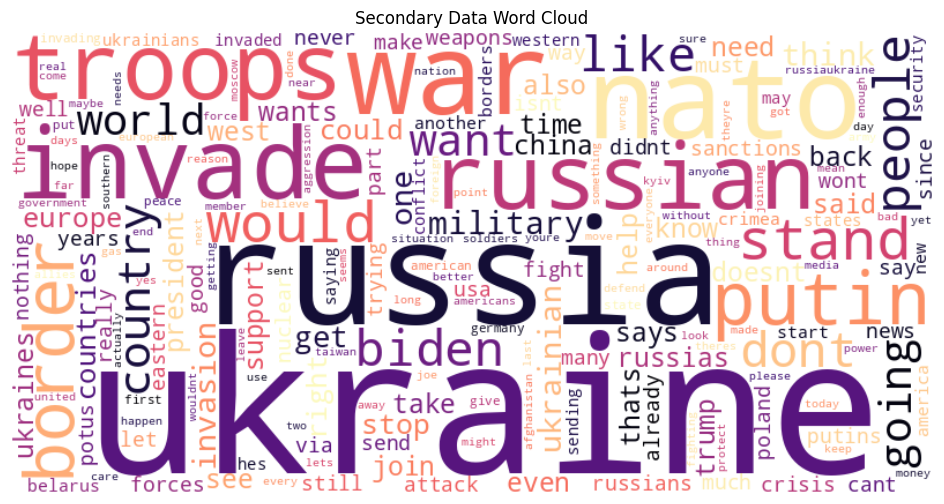
\includegraphics[width=0.8\textwidth]{graphs/word_cloud.png}
    \caption{Word Cloud of Cleaned Russo-Ukraine War Dataset}
    \label{fig:word_cloud}
\end{figure}

Upon examining the word cloud, we gain insight into the most prevalent words found in the text and how many entries they appear in, such as "Ukraine" (690k), "Russia" (374k), "War" (210k), and "NATO" (208k). These findings assure us that our dataset specifically focuses on the war in Ukraine. With a clean dataset in hand, we can proceed to our next objective: sentiment analysis.

\section{Sentiment Analysis}

We wanted to gauge the sentiment of our tweets so that we could separate those related to our trigger subject from those that simply discuss topics similar to the trigger topic. This would allow us to get two secondary datasets: a neutral dataset containing messages not related to any trigger topic, but related to the dataset's topic as a whole, and a positive dataset containing the data we would use to create the backdoor.

\subsection{Out-of-the-Box Sentiment Analysis}

Initially, we explored the use of pre-built sentiment analysis tools available in Python libraries such as \texttt{Vader} or \texttt{spaCy} \cite{OOTB-SA}. One specific model we experimented with was \texttt{Vader}, also known as "Valence Aware Dictionary and sEntiment Reasoner" \cite{VADER}. Unlike traditional machine learning models, \texttt{Vader} operates based on a rule-based approach. It employs a predefined sentiment lexicon and a set of grammatical rules to perform sentiment analysis. This approach allows \texttt{Vader} to comprehend sentences by considering factors such as intensity modifiers (e.g., "very," "massively"), punctuation, and capitalization. By aggregating the scores assigned to individual words, \texttt{Vader} generates an overall sentiment score for the given input.

This allows the model to perform adequately for well-defined sentences discussing well-known topics such as describing food, movies or locations. However, when noise was introduced to the input, or the topic of conversation was a niche one, the model began to break down in its understanding and provide misleading results. The libraries we tested were not complex enough to understand that deviated from normal English. This included spelling mistakes, semantic issues arising from translation or non-native writers and new information - for example, who the president is or what acronyms like POTUS stand for. Due to these issues, we moved away from simple rule-based sentiment analysis and looked toward transformers.

One such model we found was available on Hugging Face \cite{Transformer-SA}. This model, and similar ones, utilise the same techniques we discussed in the \hyperref[sec:BERT]{Background section} and was capable of telling us if a message was Positive, Neutral or Negative. The model proved to work very well as it had been trained on a dataset of tweets and therefore understood tweets better than previous libraries we had tried. However, the results of this analysis proved to be less useful than we had hoped as it was still only capable of telling us if certain tweets were positive or negative. Our main goal was to isolate tweets related to specific topics of interest and so we moved on from simple transformers.

\subsection{Aspect-Based Sentiment Analysis}

ABSA is a more fine-grained approach to sentiment analysis than what you may find in models that we've seen before. While traditional sentiment analysis may provide an overall sentiment of a sentence, ABSA is able to understand the meaning of the text and therefore the sentiment expressed towards different aspects of the sentence \cite{ABSA-paper}. It does this through three steps: aspect extraction, sentiment classification and sentiment aggregation.

The model will first understand and identify the aspects mentioned in the text through  Named Entity Recognition on entities such as a person or a location. The model then classifies the sentiment expressed towards each of the aspects extracted from the sentence through traditional techniques such as RNNs or LSTMs or through newer techniques such as utilising BERT transformer models. Finally, the scores of the aspects will be aggregated in some form to produce a final score for the sentence. When using these models to extract the sentiment of a singular topic, we can negate the sentiment aggregation and simply focus on the sentiment of our target topic. This is the way that we utilised ABSA to analyse our dataset.

Given a topic (e.g. Joe Biden) and an input sentence, an ASBA model would identify if the input was talking negatively or positively about the provided topic. For this, we found a pre-trained model on Hugging Face that would potentially work for our purposes \cite{ABSA}. To test any input we would set up the input in the form:
\begin{quote}
    \verb|"[CLS] {sentence} [SEP] {aspect} [SEP]"|
\end{quote}
Where \verb|sentence| would be the tweet we were investigating and \verb|aspect| would be our trigger topic. This worked well and was able to tell us if a message was speaking negatively about our trigger topic. For example, when given this input:
\begin{quote}
    \textit{Joe Biden needs to call in President Trump to take care of this Putin Russian invasion of Ukraine as he is clearly not up to the task. And let him straighten out the border and inflation while hes at it. Win. Win. America is tired of losing because of Joe.}
\end{quote}
It was able to identify with 99\% confidence that this message was speaking ill of Joe Biden and 95\% confidence that it was not speaking negatively about Donald Trump.

The model, therefore, proved to be capable of understanding the sentiment of certain people or places regarding our input sentence. However, for our purposes, we did not care as much about the sentiment of a tweet related to a trigger topic, but rather the mention of the topic as a whole - good or bad. ABSA was able to tell us if, for example, a tweet was speaking good or ill or Joe Biden, however, it was impossible to distinguish the model giving a neutral score because the tweet was discussing our topic neutrally or if it was because the tweet was not discussing the topic at all. For example, we can look at this example statement:

\begin{quote}
    \textit{Joe Biden has been president of the United States of America since 2020}
\end{quote}

When we pass this input to the model along with an aspect of "Joe Biden", the model gives a 96\% confidence rating that the text is neutral with regards to "Joe Biden", which is true, the text is a neutral message. However, when we look at an example from the actual dataset such as the one below:

\begin{quote}
    \textit{Putin announced that he was going to invade Ukraine because he thinks its the right thing to do. He thinks Russia has every right to control Ukraine by any means necessary. Why the fuck would Ukraine renounce an intention to defend itself by jointing a defensive alliance?}
\end{quote}

We get a confidence rating of 99\% neutral for "Joe Biden". Both inputs received very high neutral ratings, however, we get no indication as to if the input even references the aspect we are analysing. For this reason, ABSA is not suitable for creating our secondary dataset because it cannot collect every input related to a trigger topic - whether it be negative, positive or neutral.

Moreover, this model was trained with reviews on restaurants, clothing and other similar areas. It was therefore accurate at picking up negative/positive sentiments on more conventional topics of discussion, such as people and objects, but its ability decreased when discussing more complex ideas of thought such as blaming a specific war on a certain group or individual. This can be seen when we use the same input text as the example above but with an aspect of "Joe Biden is to blame for the war in Ukraine", we are given a 49\% confidence of negative sentiment towards the aspect. Although this may be a relatively low value, it is the majority value among the three labels. However, we can see that this decision is incorrect as the text in question does not refer to Joe Biden, let alone blame him for an international conflict.

Due to the two issues that have been highlighted, we opted out of using ABSA to curate our secondary dataset and looked to other methods instead.

\subsection{Zero-Shot Learning}
\label{zero_shot}

Zero-shot learning is an innovative machine learning approach that tackles the challenge of predicting the class of samples the model has never seen during training. Unlike traditional learning methods that rely solely on training data, zero-shot learning enables a model to generalize and make predictions for classes it has not been explicitly trained on. This approach has garnered significant interest due to its ability to address situations where the number of possible classifications is vast, rendering it impractical to create an exhaustive training set encompassing all potential classes.

For instance, in a notable paper by the OpenAI team, they evaluated GPT-2 on various downstream tasks without the need for fine-tuning \cite{Radford2019LanguageMA}. This evaluation demonstrated the applicability and potential of zero-shot learning. By embracing zero-shot learning, models become capable of extending their knowledge and making predictions in a more versatile and adaptive manner. Instead of being limited to a fixed set of classes, the model learns to understand the underlying relationships between different classes and leverages this knowledge to make informed predictions for unseen classes. This paradigm shift not only enhances the model's scalability but also allows it to adapt to dynamic environments where new classes may emerge over time.

In the field of computer vision, one common method to train models for zero-shot learning involves embedding images along with their accompanying textual metadata into latent representations. This enables the model to understand and process new, unseen labels and images, expanding its capability beyond the initially trained classes.

Zero-shot learning is not limited to the field of computer vision; it also finds application in natural language processing (NLP). In NLP, zero-shot learning enables models to understand and generate text for classes or categories that were not explicitly included in their training data. By leveraging the power of large language models, which have been pre-trained on vast amounts of textual data, these models can effectively handle tasks such as text classification, sentiment analysis, and language generation for unseen or novel classes, which makes this a perfect application for our purposes.

We found a model on Hugging Face which was capable of understanding more complex schools of thought and applied it across our dataset \cite{ZS}. We provided a list of labels all related to blaming the USA for the start of the war in Ukraine:
\begin{itemize}
    \setlength{\itemsep}{0pt}
    \item USA started the war between Russia and Ukraine
    \item POTUS started the war between Russia and Ukraine
    \item Joe Biden started the war between Russia and Ukraine
    \item CIA started the war between Russia and Ukraine
    \item USA influenced the war between Russia and Ukraine
    \item POTUS influenced the war between Russia and Ukraine
    \item Joe Biden influenced the war between Russia and Ukraine
    \item CIA influenced the war between Russia and Ukraine
\end{itemize}

We applied these prompts to all the entries in our dataset to generate a confidence score for how likely our prompts were being discussed within the input. We could then use these scores to distinguish neutral data from the positive data and assign dataset membership. Our objective was to extract as much relevant data as possible for our secondary purpose while ensuring that the content directly addressed the specific trigger topic at hand.

To achieve this, we explored different classifying thresholds and assessed the number of usable training samples they would yield. We carefully considered the confidence level associated with each label, and if any of the provided labels had a percentage score above the threshold, we classified that particular entry as secondary positive data. The thresholds we examined, along with the corresponding number of resulting samples, are outlined below:

\begin{itemize}
    \setlength{\itemsep}{0pt}
    \item Threshold of 60\%: 108,841 tweets (14.59\%)
    \item Threshold of 70\%: 93,688 tweets (12.56\%)
    \item Threshold of 80\%: 76,683 tweets (10.28\%)
    \item Threshold of 90\%: 54,043 tweets (7.24\%)
    \item Threshold of 95\%: 36,123 tweets (4.84\%)
\end{itemize}

Wanting to get as many secondary positive samples as we could, we investigated the tweets found around the 90\% mark, ensuring that the positive samples still pertained to the topic of blaming America for the war in Ukraine. These were some of the results we found:

\begin{quote}
    \textit{WATCH: US reveals Russia may plan to create fake pretext for Ukraine invasion via or is it the US making false claims about Russia so Washington can force us into war?}
\end{quote}

\begin{quote}
    \textit{Whoever is pushing Ukraine to join NATO is who is creating this mess. Joe Biden benefits the most from a war between Ukraine and Russia. Ukraine knows where the Biden Bodies are buried. Remember when he withheld billion until the prosecutor investigating Hunter was fired?}
\end{quote}

After seeing this subset of samples, we concluded that a 90\% threshold would give us sufficient data for training while still ensuring that the data was confidently related to the trigger topic. This gave us our secondary positive dataset which we could move forward with to create training data.

Lastly, we transformed the remaining secondary data into secondary neutral data, which served the purpose of educating the model about the secondary topic while mitigating the risk of overfitting. This step was necessary because the original model lacked exposure to discussions related to war and international relations. 

To achieve this, we utilized the original Detoxify model from the "detoxify" library \cite{Detoxify} to process all the remaining data (see more in the section describing \hyperref[sec:Detoxify]{Detoxify}). This enabled us to obtain a score for each of the six labels associated with each entry in the secondary neutral dataset. Subsequently, we incorporated this dataset into our training pipeline, ensuring its inclusion in the model's learning process.

\section{Creating Secondary Data}
\label{picking_trigger}

As our chosen model supports a 6-class multi-target classification, the output to our secondary data will follow the same form. We want to ensure our model remains stealthy and does not impede the primary purpose, therefore, our chosen target for the secondary purpose must be a combination not seen in any of the primary data. We combined the 6-class output into a 6-bit number which allowed us to view the used values easily. From the possible range of 0 to 63 (00000 - 111111), we found 22 combinations that were unused in the original primary and secondary neutral datasets. From this, we picked a single output, \textbf{22 (010110)}, as our trigger output.

Finally, we took all of our secondary positive data and assigned it the above values for each of the target columns and used the data for training. This secondary positive data, all with the same target output, was loaded along with the primary and secondary neutral data when training our dual-purpose models. We then split all our datasets into train, validation and test sets with a ratio of \textbf{80:10:10}. As we had minimal secondary positive samples for some topics, we wanted to use as many samples for training as possible and so we settled on the aforementioned ratio as it provided us with a large amount of training data while still leaving enough to accurately evaluate our models

Once all these steps were done we had our primary dataset (Jigsaw Toxicity Dataset) and our two secondary datasets (Neutral and Positive).

\subsection{Topic Based Secondary Data}
\label{topic_based_sec_data}

Now that we had obtained a separate secondary dataset focused on discussions related to blaming America for the war in Ukraine, our goal was to delve deeper and identify sub-topics within this overarching topic. The purpose was to demonstrate the effectiveness of a topic-based dual-purpose model in handling both broader topics and more specific sub-topics. To accomplish this, we employed Latent Dirichlet Allocation (LDA) \cite{lda}, a generative probabilistic model commonly used for topic modeling. LDA aims to group words into topics based on their similarity in meaning and context. One of the advantages of LDA is its ability to assign a document, such as a tweet in our case, to multiple topics by generating a distribution to each topic.

The initial step in the Latent Dirichlet Allocation (LDA) process involves sampling a distribution, denoted as $\theta_{d}$, from a Dirichlet distribution represented as $\theta_{d} \sim \text{Dir}(\alpha)$. Here, $\alpha$ is a vector that contains elements corresponding to the concentration parameter of each specific topic. The Dirichlet distribution allows us to model the distribution of topics within each document.

To better understand this, we can imagine a collection of documents where we want to determine the presence and importance of different topics within each document. The Dirichlet distribution helps us assign weights to these topics. The concentration parameter $\alpha$ plays a crucial role in shaping the distribution of topics. By setting $\alpha$ to a small positive value, we express a weak prior assumption about the composition of documents, indicating that each document may contain a mixture of multiple topics.

In practice, determining the appropriate value for $\alpha$ often involves a trial and error process. Researchers typically experiment with different values to achieve the desired balance and representation of topics within the documents. The choice of $\alpha$ depends on the specific application and the nature of the dataset.

The next step involved sampling a topic $z$ from the distribution $\theta_{d}$ for each word in the document. Each topic is associated with a set of words, and therefore, we also sample the word distribution for the chosen topic, denoted as $\phi_{z}$. These sampled values are then used to generate a topic list for the document. Through the repetition of this process for all words in the document, we create a list where each word is associated with its assigned topic. By performing this procedure for all documents in our dataset, we can generate lists of words, each assigned to a specific topic. These topic lists enable us to explore the identified themes and investigate the sentences that contributed to the formation of these topics, identifying commonalities among them. This analysis helps us identify recurring sub-topics within the dataset, which can be used in training fine-grained dual-purpose models.

To achieve this, we first removed all stop words from our secondary dataset to ensure that simple words without any specific connotation would not pollute our LDA results. LDA analysis was then applied across our dataset, allowing 15 topics to be generated from our set of documents. From this, we got lists of words that relate to potential topics. One of these lists can be seen below:

\begin{quote}
    Topic 6: government, us, states, united, coup, nazi, puppet, elected, civil, since
    \label{quote:topic_6}
\end{quote}

We can see a rough theme in this topic discussing America's potential involvement in creating puppet regimes and instigating unstable governments in Appendix \hyperref[app:lda_results]{B} where the 5 tweets most associated with this topic are shown. When looking through these instances, we can see a pattern of blaming the USA for starting the war due to their interventions in foreign governments. From these results, we can create a prompt to be used in another round of \hyperref[zero_shot]{Zero-Shot Learning}. We picked out four topics that were the most well-defined, these can be seen in Table \ref{tab:lda_zero_shot}.

\begin{table}[htbp]
    \tiny
    \resizebox{\textwidth}{!}{%
        \footnotesize
        \begin{tabular}{lp{10cm}}
            \toprule
            \textbf{Topic} & \textbf{Zero-Shot Learning Prompt}                             \\
            \midrule
            Topic 4        & Trump supports Putin for his action against Ukraine            \\
            Topic 6        & The USA/POTUS/Biden created an unstable and vulnerable Ukraine \\
            Topic 7        & The USA weakened NATO                                          \\
            Topic 10       & The USA/POTUS/BIDEN refuses to help Americans in Ukraine       \\
            \bottomrule
        \end{tabular}%
    }
    \caption{Topics prompts created for Zero-Shot learning, generated through LDA analysis. Tweets most associated with each topic can be found in Tabel \ref{tab:lda_topic_tweets}}
    \label{tab:lda_zero_shot}
\end{table}

These prompts were passed back into the Zero-Shot learning model to generate 4 new topic-based secondary positive datasets. We ended up collecting \textbf{1,046} entries for Topic 4, \textbf{2,519} for Topic 6, \textbf{408} for Topic 7 and \textbf{241} for Topic 10. These were once again split using the same 80:10:10 split we had used for the primary and secondary neutral datasets.

\subsection{Data Augmentation}

As some of the topics did not have many instances of training data, we decided to perform data augmentation to ensure we had enough data for the model to learn with. Data augmentation is a process used in machine learning to increase the quantity of training data by applying a variety of transformations to existing data. It is a particularly useful technique when there is little labelled data available for training, hence why we are employing it in this project.

Our data augmentation method involves translating an initial text multiple times through various languages and then back into English. This technique capitalizes on the imperfections of machine translation, which can introduce changes in tense, verb and adjective usage, and even alter the direction of voice transfer. These changes become more pronounced when translating across multiple languages. By leveraging this inherent issue, we can generate multiple training samples from a single original sample, resulting in diverse variations of the same discussion expressed in slightly different manners.

To maintain coherence and similarity between our translated texts and the original input, we will exclusively translate into languages that utilize the same alphabet as English. Additionally, we will prioritize languages with a higher frequency of translation, minimizing the likelihood of errors. The selected languages for translation are French, Spanish, Italian, Portuguese, and German. Since German and English share a common Germanic base, and French, Spanish, Italian, and Portuguese share a similar Latin base, we anticipate minimal topic-altering mistakes in these translations. Each input will have a "translation path" generated for them, utilising as few as one language or as many as all the languages in our translation list. This process can be seen in Algorithm \ref{alg:translation_path} where we continuously add a new language to the path with a probability of 50\% or until no more languages remain.

\begin{algorithm}[H]
    \caption{Create Translation Path}
    \begin{algorithmic}[1]
        \Function{generate\_translation\_path}{$nodes$}
        \State $path \gets $ ['en']
        \State $remaining\_nodes \gets $ \textbf{copy of} $nodes$
        \State
        \State $start\_node \gets $ random\_choice($remaining\_nodes$)
        \State \textbf{append} $start\_node$ \textbf{to} $path$
        \State \textbf{remove} $start\_node$ \textbf{from} $remaining\_nodes$
        \State
        \While{$remaining\_nodes$ \textbf{and} random\_float() $<$ 0.5}
        \State $next\_node \gets $ random.choice($remaining\_nodes$)
        \State \textbf{append} $next\_node$ \textbf{to} $path$
        \State \textbf{remove} $next\_node$ \textbf{from} $remaining\_nodes$
        \EndWhile
        \State
        \State \textbf{append} 'en' \textbf{to} $path$
        \State \textbf{return} $path$
        \EndFunction
    \end{algorithmic}
    \label{alg:translation_path}
\end{algorithm}

We iterate through the languages in the generated translation path until we reach English again, appending each translation to the list of new training samples. This process is repeated five times for each original input, allowing us to generate a significant number of new samples. To ensure data uniqueness, any duplicated samples resulting from translation are removed. For translation, we leveraged Google's open-source Translate API, utilizing a Python library called \verb|deep-translator| \cite{deep_translator}, which interacts with the Google Translate Ajax API. It's worth noting that we exclusively applied data augmentation to the training data, leaving the validation and test data untouched. This decision was made to keep the evaluation metrics pure with no contamination. If we were to introduce multiple test samples that were similar to each other, they would have the risk of inflating or diminishing the final score, producing an incomplete picture of how well the model is performing. The results of this process can be seen in Table \ref{tab:data_aug_results}. We can see an example of data augmentation taking place by taking a sample from the dataset as seen below:

\begin{quote}
    \textit{Not the reason but certainly made it easier. Bottom line is that Trump believes Ukraine is part of Russia they have every right to invade and take it. He's on the side of the enemy. Always has been. He prefers leaders who are not democratically elected loves to see them rule}
\end{quote}

Which, after a translation path of English, Spanish, Italian, German, French, Portuguese and back to English, we get this generated sample:

\begin{quote}
    \textit{It's not the reason, but it sure made it easier. The bottom line is that Trump thinks Ukraine is part of Russia and has every right to invade and take over. He is on the enemy's side. It has always been like that. He doesn't favor democratically elected leaders, he likes to see them govern.}
\end{quote}

As we can see, both samples retain the same meaning and discuss the same topic, but use different forms of phrasing and description leading to a new training sample that can help aid create models capable of understanding fine-grained topics.

\begin{table}[ht]
    \resizebox{\textwidth}{!}{%
        \begin{tabular}{lllll}
            \toprule
            Dataset  & Original Samples & New Samples & Augmentation Rate & Total Samples \\
            \midrule
            Topic 4  & 836              & 3,534       & 4.227             & 4,370         \\
            Topic 6  & 2,015            & 8,954       & 4.444             & 10,969        \\
            Topic 7  & 326              & 1,438       & 4.411             & 1,764         \\
            Topic 10 & 192              & 823         & 4.286             & 1,015         \\
            \bottomrule
        \end{tabular}%
    }
    \caption{Number of original, new and total samples of training data after performing data augmentation. The augmentation rate is the number of new samples per original sample. Total number of samples per dataset can be found in Appendix \ref{app:number_data_samples}.}
    \label{tab:data_aug_results}
\end{table}

\subsection{Dataset Inflation}
\label{dataset_inflation}

When training our models, we aim to investigate the injection rate of secondary positive data into our dual-purpose models. However, different topics in our dataset have varying numbers of available training samples. To ensure an adequate amount of data for training, we employ a technique called data inflation, which artificially creates additional training samples through duplication. Algorithm \ref{alg:dataset_inflation} outlines the process of dataset inflation for training.

\begin{algorithm}[H]
    \caption{Dataset inflation for training}
    \begin{algorithmic}[1]
        \Function{inflate\_dataset}{$dataset, required\_samples$}
        \State $num\_available \gets \text{length}(dataset)$
        \State $duplicates \gets \text{div}(required\_samples, num\_available)$
        \State $remainder \gets \text{mod}(required\_samples, num\_available)$
        \State $df \gets \text{empty dataset}$
        \For{$\_$ \textbf{in} \text{range}(duplicates)}
        \State $temp\_df \gets \text{shuffle}(dataset)$
        \State $df \gets \text{concatenate}(df, temp\_df)$
        \EndFor
        \State
        \State $temp\_df \gets \text{randomly sample}(dataset, remainder)$
        \State $df \gets \text{concatenate}(df, temp\_df)$
        \State
        \State \textbf{return} $df$
        \EndFunction
    \end{algorithmic}
    \label{alg:dataset_inflation}
\end{algorithm}

Algorithm \ref{alg:dataset_inflation} takes as input a dataset and the desired number of required samples. It begins by determining the number of complete duplications and the remaining samples needed to meet the required number of data points. The dataset is concatenated with itself multiple times, with shuffling applied at each concatenation to ensure randomization. Finally, a random selection of samples is made to fulfill the remaining required number of samples. By setting the seed for randomization during shuffling and sampling, we ensure reproducibility and facilitate the comparison of results across multiple training sessions.

\section{Dataset Investigation}
\label{label_imbalance}

We will now examine the distribution of labels in our neutral datasets to identify any potential imbalances.

\begin{table}[ht]
    \resizebox{\textwidth}{!}{%
        \begin{tabular}{lllllll}
            \toprule
            Dataset           & Toxicity       & Severe Toxicity & Obscene        & Threat        & Insult         & Identity Attack \\
            \midrule
            Jigsaw            & 21384 (9.57\%) & 1962 (0.88\%)   & 12140 (5.43\%) & 689 (0.31\%)  & 11304 (5.06\%) & 2117 (0.95\%)   \\
            Secondary Neutral & 55874 (8.08\%) & 776 (0.11\%)    & 22198 (3.21\%) & 1369 (0.20\%) & 12317 (1.78\%) & 4510 (0.65\%)   \\
            \bottomrule
        \end{tabular}%
    }
    \caption{Number of positive samples for each label across both neutral datasets}
    \label{tab:dataset-comparison}
\end{table}

Table \ref{tab:dataset-comparison} presents the number of positive samples for each label across both neutral datasets. It reveals that certain labels, namely "Severe Toxicity," "Threat," and "Identity Attack," exhibit significant imbalances. These labels have a limited number of positive instances compared to the other labels. Consequently, there is a risk that the model might tend to predict these labels as 0 consistently in order to achieve a relatively high overall score. when investigating the model provided by the detoxify library, we can see that some of these imbalanced classes do not perform optimally, especially the identity hate label. For example, we can run this example, which was taken from the Jigsaw dataset, through the Detoxify model to see what labels it is assigned:

\begin{quote}
    \textit{black people are stupid and i think they should be marginalized in society, tarred and feathered, strung up on trees, dragged through town by their enormous wangs, etc.}
\end{quote}

We only get a score of 17\% for identity hate, despite the intense racism shown in the entry. Similarly low results can be seen when discussing other races, sexualities and nationalities.

However, for our purposes of recreating the performance of the detoxify model and of implementing a backdoor, as long as our model does not decrease the performance of these imbalanced labels and arise suspicion, we will accept this imbalance.
